% !TeX program = pdflatex
% Compile with: latexmk -pdf -interaction=nonstopmode main.tex
\documentclass[11pt,a4paper]{article}

\usepackage[T1]{fontenc}
\usepackage[utf8]{inputenc}
\usepackage[scaled=0.95]{helvet}
\renewcommand{\familydefault}{\sfdefault}
\usepackage{newunicodechar}
\newunicodechar{š}{\v{s}}
\newunicodechar{ũ}{\~{u}}
\usepackage{microtype}
\usepackage[a4paper,margin=22mm,headheight=22pt]{geometry}
\usepackage{amsmath,amssymb,mathtools}
\usepackage{booktabs,longtable,array,tabularx}
\usepackage{ragged2e}
\usepackage{pdflscape}
\usepackage{float}
\usepackage[table]{xcolor}
\usepackage{enumitem}
\usepackage{fancyhdr}
\usepackage{titlesec}
\usepackage{csquotes}
\usepackage{graphicx}
\usepackage{hyperref}
\usepackage{bookmark}
\ifdefined\CoverOnlyBuild
\else
  \usepackage[
    backend=biber,
    style=authoryear,
    sorting=nyt,
    maxcitenames=2,
    maxbibnames=99,
    giveninits=true,
    uniquename=init,
    doi=true,
    url=true,
    eprint=true
  ]{biblatex}
  \addbibresource{references.bib}
\fi

% Shared with the microsite: charcoal ink, quiet grey rules, and one link blue.
\definecolor{Navy}{HTML}{424242}
\definecolor{Teal}{HTML}{2A7AE2}
\definecolor{PaleBlue}{HTML}{F6F6F6}
\definecolor{PaleGold}{HTML}{F6F6F6}
\definecolor{PaleGray}{HTML}{F6F6F6}
\definecolor{MidGray}{HTML}{828282}
\definecolor{RuleGray}{HTML}{E8E8E8}

\hypersetup{
  colorlinks=true,
  linkcolor=Teal,
  citecolor=Teal,
  urlcolor=Teal,
  pdftitle={AI and Mathematical Proof: From a Sparse 2025 Baseline to the 2026 Take-off},
  pdfauthor={OpenAI},
  pdfsubject={Automated theorem proving and AI-assisted mathematical discovery}
}

\titleformat{\section}{\Large\normalfont\color{Navy}}{\thesection}{0.65em}{}
\titleformat{\subsection}{\large\bfseries\color{Navy}}{\thesubsection}{0.65em}{}
\titlespacing*{\section}{0pt}{2.0ex plus .4ex}{0.8ex}
\titlespacing*{\subsection}{0pt}{1.4ex plus .3ex}{0.6ex}

\pagestyle{fancy}
\fancyhf{}
\lhead{\small\color{Navy}SuperLattice}
\rhead{\small\color{MidGray}January 2025--21 July 2026}
\cfoot{\small\thepage}
\renewcommand{\headrulewidth}{0.4pt}
\renewcommand{\headrule}{\hbox to\headwidth{\color{RuleGray}\leaders\hrule height \headrulewidth\hfill}}

\setlist[itemize]{leftmargin=1.35em,itemsep=0.20em,topsep=0.35em}
\setlist[enumerate]{leftmargin=1.55em,itemsep=0.20em,topsep=0.35em}
\setlength{\parindent}{0pt}
\setlength{\parskip}{0.45em}
\setlength{\emergencystretch}{2em}

\newcommand{\K}{\textbf{K}}
\newcommand{\Hc}{\textbf{H}}
\newcommand{\Sg}{\textbf{S}}
\newcommand{\Prv}{\textbf{P}}
\newcommand{\entry}[1]{\textbf{#1}}
\newcolumntype{L}[1]{>{\RaggedRight\arraybackslash}p{#1}}
\newcolumntype{C}[1]{>{\Centering\arraybackslash}p{#1}}
\newcommand{\covernotice}[3]{%
  \begingroup
  \setlength{\tabcolsep}{0pt}%
  \noindent
  \begin{tabular}{@{}>{\columncolor{#1}}p{3pt}@{}>{\columncolor{PaleGray}}m{\dimexpr\textwidth-3pt\relax}@{}}
    \rule{0pt}{#2} & \hspace*{4mm}\parbox{\dimexpr\linewidth-8mm\relax}{#3}\hspace*{4mm}
  \end{tabular}%
  \endgroup
}
\newcommand{\ExpectedCount}{8}
\newcommand{\DifficultCount}{28}
\newcommand{\SuperhumanCount}{28}
\newcommand{\MeanDifficultyScore}{3.7}
\newcommand{\TotalScoredEntries}{64}


\begin{document}
\hypersetup{pageanchor=false}
\begin{titlepage}
\thispagestyle{empty}
{\color{Navy}\rule{\textwidth}{3.5pt}}\\[8mm]
{\fontsize{18}{22}\selectfont\color{Navy} SuperLattice}\hfill
{\small\color{MidGray}Research report}\\[7mm]
{\color{RuleGray}\rule{\textwidth}{0.5pt}}\\[15mm]
\noindent
\begin{minipage}[b]{0.59\textwidth}
\RaggedRight
{\small\color{MidGray}Research project \textperiodcentered\ Evidence through 21 July 2026}\par\vspace{3mm}
{\fontsize{30}{34}\selectfont\color{Navy} AI and mathematical\\proof progress}\par\vspace{4mm}
{\fontsize{14}{19}\selectfont\color{Navy} From a sparse 2025 baseline to the\\2026 take-off}\par\vspace{3mm}
{\fontsize{10.5}{15.5}\selectfont\color{MidGray}An exploratory record of audited AI contributions to automated and semi-automated mathematical proofs, constructions, bounds and counterexamples.}\par
\end{minipage}
\hfill
\begin{minipage}[b]{0.35\textwidth}
\raggedleft
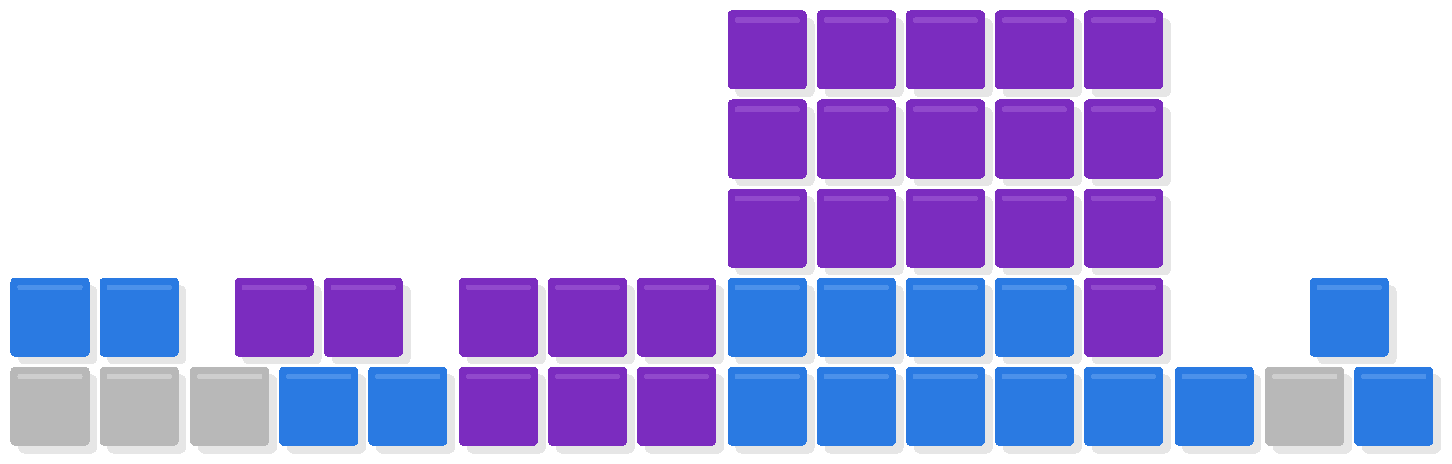
\includegraphics[width=\linewidth]{data-city.pdf}
\end{minipage}
\vspace{11mm}

\covernotice{MidGray}{29mm}{%
  {\fontsize{9.5}{13.5}\selectfont
  \textbf{AI analysis disclaimer}\par\vspace{1.5mm}
  This is an AI-assisted analysis, not an expert-reviewed census. The evidence collection was last run through \textbf{21 July 2026} and contains \textbf{64 audited entries}. The supplied source bundle does not record which model produced the baseline collection. This dashboard and hybrid-scoring rerun were prepared with \textbf{OpenAI Codex, based on GPT-5}. Treat the classifications as reproducible proxies and check substantive claims against the cited works.}}

\vspace{7mm}
{\small
\begin{tabularx}{\textwidth}{@{}L{39mm}>{\RaggedRight\arraybackslash}X@{}}
\textbf{Evidence window} & 1 January 2025 to 21 July 2026. \\
\textbf{Research ledger} & Twenty entries first reported in 2025 plus 44 entries first reported in 2026. \\
\textbf{Counting rule} & A month receives an entry only for a new public mathematical conclusion, best-known bound, counterexample, or bounded construction portfolio with a documented AI contribution and a checkable source. \\
\textbf{Zero-month rule} & Zero means that this audit found no public item meeting the threshold. It does not prove that no private, unreported, or differently classified AI-assisted work occurred. \\
\end{tabularx}
}
\vfill
\covernotice{Teal}{19mm}{%
  {\fontsize{9.5}{13.5}\selectfont
  \textbf{Central finding.} January--March 2025 form a flat audited baseline. Isolated discoveries begin in April and May, June--July are flat again, and a broader August--December ramp precedes the much larger portfolio-production surge of spring 2026.}}
\end{titlepage}
\ifdefined\CoverOnlyBuild
  \end{document}
\fi
\hypersetup{pageanchor=true}
\pagenumbering{roman}
\tableofcontents
\clearpage
\pagenumbering{arabic}

\section{Executive summary}

Extending the audit to January 2025 makes the take-off pattern clearer without manufacturing a false zero baseline. The strict ledger contains no qualifying public entries in \textbf{January, February, or March 2025}; one appears in April and one in May; June and July are again zero; two appear in August; six in September; and ten across Q4. The year therefore closes at 20 entries. The ledger then reaches 35 by the end of April 2026, 60 by the end of May, and 64 by 21 July.

The curve measures \emph{audited public result packages}, not unique problems or every theorem statement. AlphaEvolve, ThetaEvolve, and the AlphaProof Nexus OEIS result are aggregate rows, while independent result packages addressing the same target remain separate. The supplied ledger was intended to exclude benchmarks, contest solutions, formalizations of already-known mathematics, rediscoveries, and papers reporting only partial proof fragments. This scoring rerun holds its 64 rows fixed so that corpus revision is not mixed with metric revision; the entry-level rationales flag two later-documented prior-result cases (IDs 23 and 32).

The chronology supports three phases: a sparse early baseline; an ignition period from April through Q4 2025; and a production take-off in spring 2026, when systems began combining retrieval, parallel search, counterexample generation, statement repair, formal verification, and expert review into repeatable pipelines. May 2026 alone contributes 25 entries, 39.1\% of the full ledger.

\section{Scope and evidence labels}

The intended inclusion rule is conservative. A qualifying entry requires: (i) a public source dated within the evidence window; (ii) a new mathematical outcome or improved best-known construction; (iii) a material, documented AI role; and (iv) human or machine verification sufficient to audit the claim. The present rerun reclassifies the supplied ledger rather than silently deleting rows when later source review changes a novelty judgment. The absence of entries in a month therefore means ``no qualifying item located in this curated audit,'' not ``no AI mathematics activity.''

\begin{tabularx}{\textwidth}{@{}C{10mm}L{28mm}X@{}}
\toprule
\textbf{Code} & \textbf{Meaning} & \textbf{Interpretation}\\
\midrule
\K & Kernel-checked & A proof assistant accepts a fully formal statement. This checks deduction, not novelty or semantic fidelity by itself.\\
\Hc & Human-checked & Domain experts report checking, completing, or rewriting the argument.\\
\Sg & Specialist digest & An external specialist has published a clarification, rewrite, or companion account.\\
\Prv & Provisional & Very recent claim or incomplete independent validation at the cut-off.\\
\bottomrule
\end{tabularx}

\section{Challenge categories}

The companion microsite adds a three-tier classification to distinguish lower-scoring entries from results with more documented challenge signals. Every entry receives the same source-grounded hybrid score
\[
D=P+A+S+R, \qquad 0\le D\le5,
\]
where $P$ records a documented prior target, $A$ scores the mathematical advance from 0 to 2, $S$ records uniform or genuinely general scope, and $R$ records demonstrated resistance. Each component is awarded once from the paper and cited prior work, not accumulated from keywords in a summary.

The design draws on three useful precedents without pretending they are interchangeable. TPTP records observed failure across state-of-the-art provers \parencite{SutcliffeSuttner2001ATP}. FrontierMath separately reviews background, insight, and execution \parencite{GlazerEtAl2025FrontierMath}. The literature also measures elapsed time from precise conjecture formulation to proof \parencite{HisanoSornette2013TimeToProof}. Comparable solver matrices and expert-hour estimates are unavailable for most research papers, so these precedents inform the rubric and the optional resistance component rather than becoming mandatory fields.

\begin{table}[H]
\small
\renewcommand{\arraystretch}{1.16}
\begin{tabularx}{\textwidth}{@{}L{22mm}L{32mm}X@{}}
\toprule
\textbf{Component} & \textbf{Points} & \textbf{Operational rule} \\
\midrule
$P$: prior target & 0--1 & One point only when the exact question, conjecture, record, or quantitative frontier is documented in a source predating the AI-assisted work. \\
\rowcolor{PaleBlue}
$A$: advance & 0--2 & Zero for a narrow or unquantified extension; one for a material improvement, new theorem, construction, counterexample, or substantial subcase; two for complete proof or disproof, classification, matching optimum, sharp endpoint, or removal of the central condition. \\
$S$: scope & 0--1 & One point for a uniform or worst-case result over an unbounded or genuinely general class, rather than a fixed object, finite list, or undifferentiated portfolio. \\
\rowcolor{PaleBlue}
$R$: resistance & 0--1 & One point for at least two independent pre-solution attacks on the exact target, or a predeclared target-specific comparison with at least five independent runs or systems and no more than 20\% success. \\
\bottomrule
\end{tabularx}
\caption{Operational components of the hybrid challenge score.}
\end{table}

Scores of 0--2 are labelled \textbf{Expected}; scores of 3--5 are labelled \textbf{Difficult}. \textbf{Superhuman} overrides the base label only when $P=1$, $A=2$, the claim is non-provisional, and at least 1.0 decade elapsed from the earliest precise framing of substantially the same target to its solution. Here $A=2$ operationalizes complete settlement of the anchor claim; it is not a publication-status judgment. Duration is derived from the recorded integer years and reported in decades. Superhuman is a historical-result label, not a claim about novelty or the contributing system's general capability.

The rerun classifies \TotalScoredEntries{} result packages: \ExpectedCount{} Expected, \DifficultCount{} Difficult, and \SuperhumanCount{} Superhuman, with a mean base score of \MeanDifficultyScore{} out of 5. These are not counts of unique problems: for example, IDs 14 and 31 are independent packages addressing the same Burr--Erd\H{o}s target. Verification strength, AI autonomy, publication prestige, proof length, and compute are retained as separate evidence and do not add difficulty points. Provisional claims may receive a high base score but cannot be Superhuman. Figure~\ref{fig:takeoff} shows the monthly category mix alongside the cumulative series, and Table~\ref{tab:difficulty-scores} gives the complete entry-level audit trail.

\section{The extended take-off curve}

Figure~\ref{fig:takeoff} uses the first public report date, normally the first official release or arXiv version. The stacked bars make zero months explicit and distinguish the Expected, Difficult, and Superhuman categories; the line gives the cumulative series. The Superhuman segment records settled results whose precise target predates the solution by at least one decade. AlphaEvolve is counted in May 2025, when Google DeepMind first announced its mathematical results, rather than again when the white paper and expanded portfolio appeared.

\begin{figure}[H]
\centering
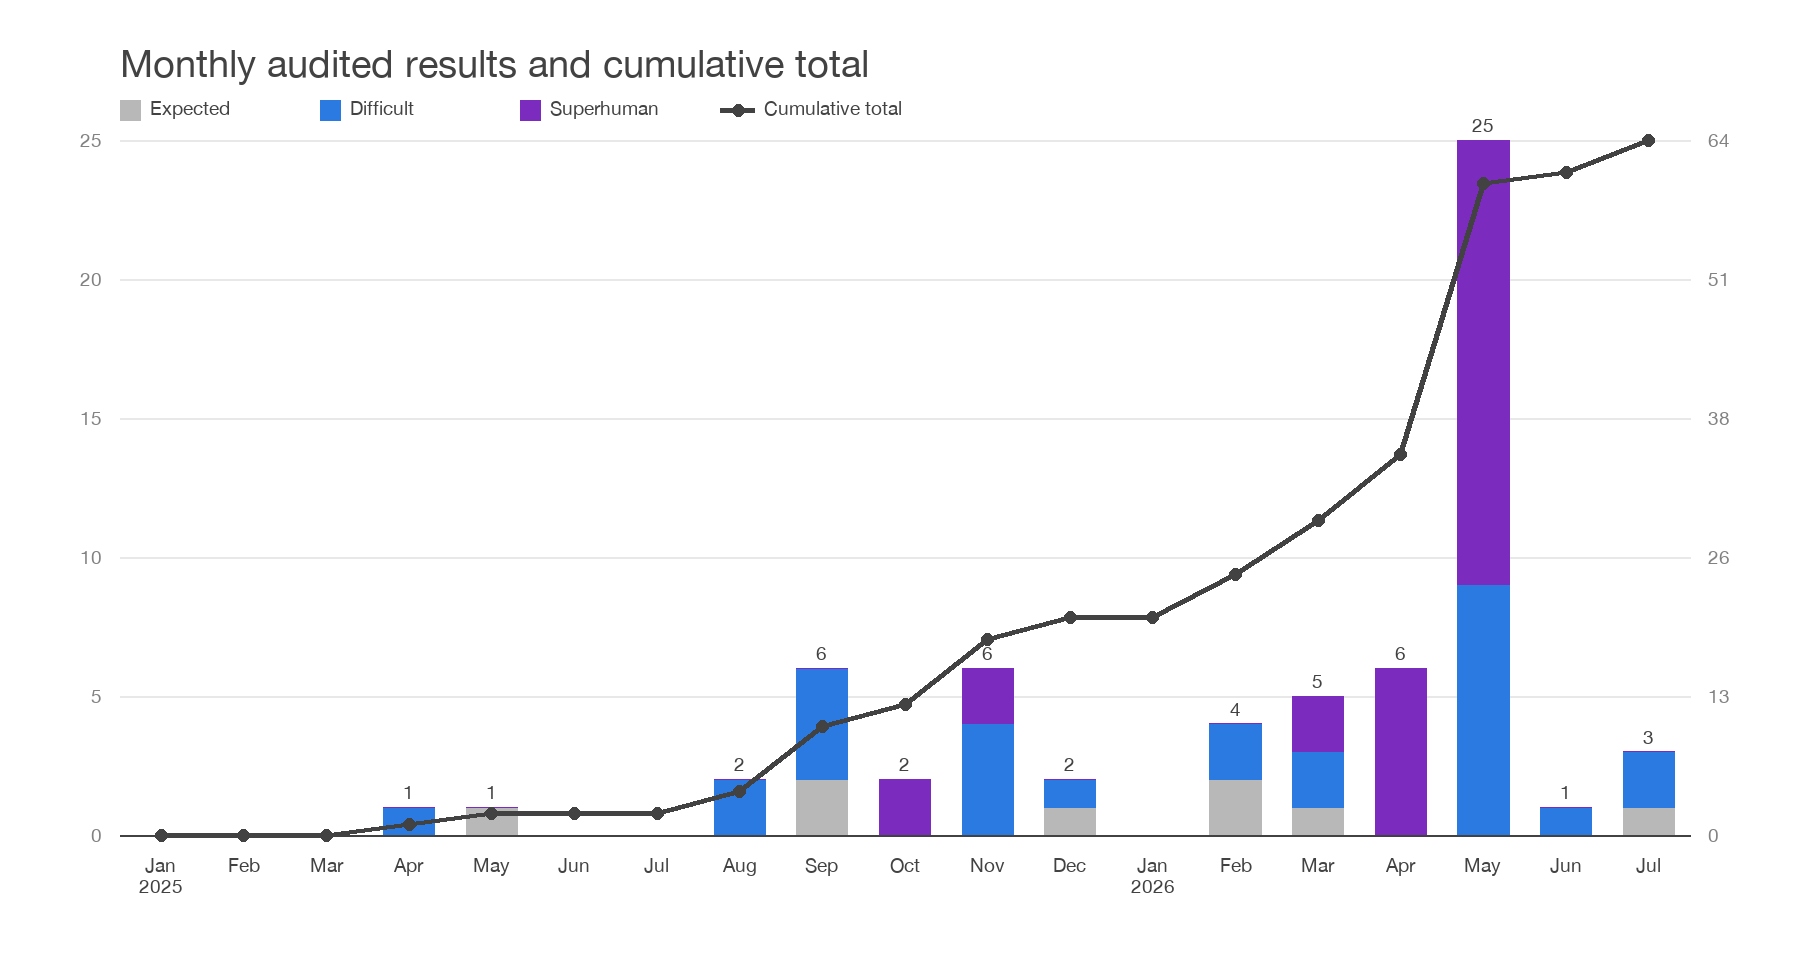
\includegraphics[width=0.96\textwidth]{cumulative_takeoff_jan2025.png}
\caption{Monthly audited research-ledger entries by hybrid challenge category, with the cumulative total, from January 2025 to 21 July 2026. July 2026 is partial. Zero bars indicate no qualifying public entry located under the report's strict threshold, not universal nonexistence.}
\label{fig:takeoff}
\end{figure}

\begin{table}[H]
\centering
\scriptsize
\renewcommand{\arraystretch}{1.10}
\begin{tabular}{@{}lrrrrrrrrrrrr@{}}
\toprule
\textbf{2025} & Jan & Feb & Mar & Apr & May & Jun & Jul & Aug & Sep & Oct & Nov & Dec \\
\midrule
New entries & 0 & 0 & 0 & 1 & 1 & 0 & 0 & 2 & 6 & 2 & 6 & 2 \\
Cumulative & 0 & 0 & 0 & 1 & 2 & 2 & 2 & 4 & 10 & 12 & 18 & 20 \\
\bottomrule
\end{tabular}

\vspace{1.5mm}
\begin{tabular}{@{}lrrrrrrr@{}}
\toprule
\textbf{2026} & Jan & Feb & Mar & Apr & May & Jun & Jul* \\
\midrule
New entries & 0 & 4 & 5 & 6 & 25 & 1 & 3 \\
Cumulative & 20 & 24 & 29 & 35 & 60 & 61 & 64 \\
\bottomrule
\end{tabular}
\caption{Underlying entry counts. ``Jul*'' ends on 21 July 2026.}
\end{table}

The flat intervals matter. They show that the 2026 rise is not an artifact of starting the graph at the first success. Yet the curve should not be over-interpreted: publication is lumpy, the audit is curated, and several rows aggregate multiple mathematical advances.

\begin{landscape}
\section{2025 precursor ledger}
\fontsize{7.35}{8.18}\selectfont
\setlength{\tabcolsep}{2.25pt}
\renewcommand{\arraystretch}{1.04}
\begin{longtable}{@{}C{10mm}C{16mm}L{68mm}L{25mm}L{22mm}L{38mm}L{46mm}@{}}
\caption{Audited 2025 research results used to establish the pre-take-off baseline.}\label{tab:2025ledger}\\
\toprule
\textbf{No.} & \textbf{First report} & \textbf{Theorem, counterexample, or construction} & \textbf{Primary area} & \textbf{Outcome} & \textbf{AI workflow} & \textbf{Verification and status} \\
\midrule
\endfirsthead
\multicolumn{7}{l}{\textit{Table \thetable{} continued from previous page}}\\
\toprule
\textbf{No.} & \textbf{First report} & \textbf{Theorem, counterexample, or construction} & \textbf{Primary area} & \textbf{Outcome} & \textbf{AI workflow} & \textbf{Verification and status} \\
\midrule
\endhead
\midrule
\multicolumn{7}{r}{\textit{Continued on next page}}\\
\endfoot
\bottomrule
\endlastfoot

25--1 & 1 Apr & \entry{Deletion-correcting code constructions.} An LLM-guided FunSearch adaptation recovered a function constructing the conjectured-optimal Varshamov--Tenengolts code for one deletion and improved prior finite constructions for multiple deletions and quaternary edit channels. \parencite{WeindelHeckel2025DeletionCodes} & Information theory / coding & Proved construction and improved finite codes & LLM-generated programs evolved against automated code-size evaluators & \Hc. The single-deletion construction is proved; the multi-deletion results are explicit computational constructions rather than a general theorem. \\
\rowcolor{PaleBlue}
25--2 & 14 May & \entry{AlphaEvolve mathematics portfolio.} The first public announcement reported new solutions or improved constructions across more than 50 open mathematical problems, including a 48-scalar-multiplication algorithm for $4\times4$ complex matrices; later technical reports expanded the portfolio. \parencite{DeepMind2025AlphaEvolve,NovikovEtAl2025AlphaEvolve,GeorgievEtAl2025AlphaEvolve} & Cross-field constructive mathematics & Improved algorithms and bounds & Evolutionary Gemini coding agents with automated evaluators & \Hc. Counted once at first public report; later papers are supporting documentation, not additional monthly entries. \\
25--3 & 11 Aug & \entry{$X$-evolve cap-set and Shannon-capacity constructions.} A larger partial admissible set raised the cap-set constant lower bound to $C\ge2.2203$, while an independent set of size 19,946 in $C_{15}^{\boxtimes5}$ raised the corresponding Shannon-capacity lower bound. \parencite{ZhaiEtAl2025XEvolve} & Extremal combinatorics / information theory & Improved lower bounds & LLMs evolved parameterized solution spaces followed by score-based search & \Hc. Explicit finite constructions in a technical preprint; grouped as one system-paper result package. \\
\rowcolor{PaleBlue}
25--4 & 16 Aug & \entry{Three-player approximate Nash equilibrium.} LegoNE discovered a polynomial-time algorithm improving the worst-case guarantee from $0.6+\delta$ to $0.5+\delta$, beyond the previously known multiplayer extension technique. \parencite{LiEtAl2025LegoNE} & Algorithmic game theory & Improved algorithm and guarantee & A reasoning LLM generated algorithms in a domain language compiled to finite certification problems & \Hc. The symbolic certificate establishes the worst-case guarantee. \\
25--5 & 3 Sep & \entry{Quantitative Malliavin--Stein fourth-moment bounds.} GPT-5 extended qualitative fourth-moment results to explicit convergence rates in Gaussian and Poisson settings, addressing a question the authors report had not previously been treated. \parencite{DiezEtAl2025MalliavinStein} & Probability theory & Proved quantitative bounds & Controlled GPT-5 research experiment with expert prompting and checking & \Hc. Expert-authored paper; no proof-assistant formalization. \\
\rowcolor{PaleBlue}
25--6 & 17 Sep & \entry{Circle packing by sample-efficient program evolution.} ShinkaEvolve reported a new best-known circle-packing construction using only 150 candidate samples. \parencite{LangeEtAl2025ShinkaEvolve} & Discrete geometry / optimization & Improved construction & LLM mutation, novelty rejection, and bandit-based model selection & \Hc. Computationally evaluated construction in an open-source system paper. \\
25--7 & 22 Sep & \entry{G\"odel Test, Problem 2.} GPT-5 derived a different approximation guarantee that refuted the authors' proposed conjecture while giving a valid replacement result. \parencite{FeldmanKarbasi2025Godel} & Combinatorial optimization & Counterexample and theorem & General-purpose GPT-5 supplied the decisive alternative analysis & \Hc. The authors checked the derivation and document both successes and failures. \\
\rowcolor{PaleBlue}
25--8 & 22 Sep & \entry{Certification on random regular graphs.} Near-optimal upper and conditional lower bounds were obtained for certifying MAX-CUT and MAX-Independent Set on random 3- and 4-regular graphs, using nearly extremal Ramanujan graphs found by AlphaEvolve. \parencite{NagdaEtAl2025Reinforced} & Complexity theory / graph theory & Sharper bounds & AlphaEvolve searched for finite graph constructions; humans supplied the analytical arguments & \Hc. Expert-authored proof with explicit AI-generated constructions and verification procedures. \\
25--9 & 22 Sep & \entry{MAX-$k$-CUT inapproximability.} New gadget reductions improve NP-hardness-of-approximation factors for MAX-4-CUT and the best gadget-based factor for MAX-3-CUT reported by the paper. \parencite{NagdaEtAl2025Reinforced} & Computational complexity & Improved hardness results & AlphaEvolve discovered and helped verify finite gadgets & \Hc. The reductions and soundness arguments are checked by the authors. \\
\rowcolor{PaleBlue}
25--10 & 25 Sep & \entry{Optimality of black-box amplification in QMA.} Doubly exponential completeness amplification is optimal for polynomial-resource black-box procedures. GPT-5 supplied a resolvent-trace idea used as a key technical step. \parencite{AaronsonEtAl2025QMA,Aaronson2025QMAAI} & Quantum complexity & Proved lower bound & Iterative human--model exchange supplied a technical construction inside a human-led proof & \Hc. Conventional expert-authored preprint; a coauthor publicly documented the model's role. \\
25--11 & 22 Oct & \entry{Majority optimality in NICD with erasures.} A five-bit unbiased Boolean function beats five-bit majority at erasure probability $p=0.40$, disproving the proposed optimality of majority. \parencite{IvanisviliXie2025NICD} & Probability / theoretical computer science & Counterexample & GPT-5 Pro searched an open-problem list and proposed the explicit function & \Hc. The note verifies the finite computation step by step by hand. \\
\rowcolor{PaleBlue}
25--12 & 27 Oct & \entry{Point convergence of Nesterov acceleration.} The standard accelerated gradient method has point convergence in the paper's convex smooth setting, resolving a question open since the method's introduction. \parencite{JangRyu2025Nesterov} & Convex optimization & Proved & ChatGPT materially assisted discovery of the proof & \Hc. Expert-authored preprint with a documented elicitation process. \\
25--13 & 20 Nov & \entry{Erd\H{o}s Problem 848.} For sufficiently large $n$, the extremal family of integers whose pairwise sums are never squarefree has the asserted maximum size, with near-uniqueness of the extremizers. \parencite{BubeckEtAl2025GPT5Science} & Combinatorial number theory & Proved & GPT-5 Pro supplied a key density idea; mathematicians corrected and completed it & \Hc. Complete expert-written proof. \\
\rowcolor{PaleBlue}
25--14 & 20 Nov & \entry{Follow-the-leader for nested convex-body chasing.} The minimum-norm rule can incur arbitrarily large cost even in two dimensions, so its competitive ratio is infinite. \parencite{BubeckEtAl2025GPT5Science} & Online algorithms / convex geometry & Counterexample & GPT-5 produced the adversarial construction from a short prompt & \Hc. Human expert corrected minor inaccuracies and presented the proof. \\
25--15 & 20 Nov & \entry{Convex-body chasing lower bounds.} A cleaner and stronger lower-bound construction for arbitrary online algorithms was obtained, with a higher-dimensional extension by orthogonal decomposition. \parencite{BubeckEtAl2025GPT5Science} & Online optimization & Improved bound & Human construction plus GPT-5's switching fix and dimension-extension idea & \Hc. Expert-written proof documenting useful and failed attempts. \\
\rowcolor{PaleBlue}
25--16 & 20 Nov & \entry{Second tree-profile inequality.} The remaining open inequality among the first two conjectured faces for induced five-vertex subtree counts is true. \parencite{BubeckEtAl2025GPT5Science} & Extremal graph theory & Proved & Scaffolded GPT-5 reproved the known first inequality, then generated the open second proof & \Hc. AI-generated proof with expert checking and editorial rewriting. \\
25--17 & 20 Nov & \entry{Identifiability in a dynamic random network.} In an attractiveness-weighted preferential-attachment tree, the hidden parameter is identifiable from one large unlabelled tree through the limiting fraction of leaves. \parencite{BubeckEtAl2025GPT5Science} & Probability / learning theory & Proved & Scaffolded GPT-5 selected the observable and supplied the main architecture & \Hc. Humans filled routine stochastic-approximation details. \\
\rowcolor{PaleBlue}
25--18 & 28 Nov & \entry{ThetaEvolve open-problem portfolio.} A single open-source 8B model improved reported bounds on circle packing and the first autocorrelation inequality. \parencite{WangEtAl2025ThetaEvolve} & Geometry / analysis / optimization & Two improved bounds & Test-time program evolution with optional reinforcement learning and automated scoring & \Hc. Aggregate portfolio entry supported by released code and a technical report. \\
25--19 & 10 Dec & \entry{Grover-compatible manifold optimization.} A human--AI workflow identified invariant subspaces, constructed compatible retractions, and established convergence guarantees for a retraction-based gradient method. \parencite{LiEtAl2025HumanAI} & Optimization / quantum computing & Theory and convergence results & LLMs searched for proofs, contradictions, structures, and parameters under expert control & \Hc. Human authors refined outputs into precise statements and rigorous proofs. \\
\rowcolor{PaleBlue}
25--20 & 16 Dec & \entry{Extremal descendant integrals.} For pure $\psi$-class intersection numbers on $\overline{\mathcal M}_{g,n}$, the minimum occurs when all but one exponent vanish, while balanced exponent vectors maximize the value. \parencite{Schmitt2025ExtremalDescendant} & Algebraic geometry & Proved & GPT-5 and Gemini 3 Pro found and formulated the proof; other models assisted drafting and formalization & \Hc, with partial \K. The paper exposes prompts, attribution, and a partial Lean development. \\
\end{longtable}
\end{landscape}

\begin{landscape}
\section{2026 research ledger (through 21 July)}
\fontsize{7.6}{8.5}\selectfont
\setlength{\tabcolsep}{3.0pt}
\renewcommand{\arraystretch}{1.05}
\begin{longtable}{@{}C{7mm}L{78mm}L{27mm}L{21mm}L{40mm}L{52mm}@{}}
\caption{Publicly documented 2026 research results with material AI contribution. Status records the evidence available by 21 July 2026.}\label{tab:ledger2026}\\
\toprule
\textbf{No.} & \textbf{Theorem, counterexample, or construction} & \textbf{Primary area} & \textbf{Outcome} & \textbf{AI workflow} & \textbf{Verification and status} \\
\midrule
\endfirsthead
\multicolumn{6}{l}{\textit{Table \thetable{} continued from previous page}}\\
\toprule
\textbf{No.} & \textbf{Theorem, counterexample, or construction} & \textbf{Primary area} & \textbf{Outcome} & \textbf{AI workflow} & \textbf{Verification and status} \\
\midrule
\endhead
\midrule
\multicolumn{6}{r}{\textit{Continued on next page}}\\
\endfoot
\bottomrule
\endlastfoot
1 & \entry{Planar unit-distance conjecture.} There are infinitely many $n$ for which an $n$-point planar set determines at least $n^{1+\delta}$ unit-distance pairs for some fixed $\delta>0$, disproving the conjectured $n^{1+o(1)}$ upper-order behavior. \parencite{OpenAIUnitDistance2026,AlonEtAl2026UnitDistance} & Discrete geometry / number theory & Disproved & General-purpose OpenAI reasoning model; no problem-specific theorem prover & \Hc+\Sg. External mathematicians checked the proof and produced a digested companion paper. Preprint, but unusually strong public expert validation. \\
\rowcolor{PaleBlue}
2 & \entry{Cycle Double Cover Conjecture.} Every finite bridgeless graph has a multiset of cycles covering every edge exactly twice. \parencite{OpenAI2026CDC,Geelen2026CDC} & Graph theory & Claimed proof & OpenAI reasoning model; short natural-language proof artifact & \Sg+\Prv. A specialist clarification exists, but the claim was only days old at the cut-off and had not completed conventional peer review. \\
3 & \entry{Anderson's quasi-completeness problem.} A weakly quasi-complete Noetherian local ring need not be quasi-complete. \parencite{JuEtAl2026RethlasArchon,JiangEtAl2026Rethlas} & Commutative algebra & Counterexample & Rethlas informal discovery + Archon formalization and proof search & \K+\Hc. End-to-end Lean 4 proof with essentially no human involvement in solving/formalizing; separately presented in a human-verified paper. \\
\rowcolor{PaleBlue}
4 & \entry{Finite conductor and group rings.} The finite-conductor property does not necessarily ascend from a G--GCD ring $R$ to $RG$ for finitely generated abelian $G$. \parencite{JiangEtAl2026Rethlas} & Commutative algebra & Counterexample & Rethlas natural-language automated reasoning & \Hc. Self-contained AI-generated proof, subsequently verified by human experts. \\
5 & \entry{Quasi-coherence and group rings.} The quasi-coherent property likewise need not ascend from a G--GCD ring to its group ring. \parencite{JiangEtAl2026Rethlas} & Commutative algebra & Counterexample & Rethlas & \Hc. AI-generated, human-verified preprint. \\
\rowcolor{PaleBlue}
6 & \entry{Integer-valued polynomial birings.} There exists an integral domain $D$ for which $\operatorname{Int}(D)$ admits no compatible $D$--$D$ biring structure of the specified kind. \parencite{JiangEtAl2026Rethlas} & Commutative algebra & Counterexample & Rethlas & \Hc. AI-generated, human-verified preprint. \\
7 & \entry{AGCD domains.} If every nonzero $t$-locally principal ideal of an almost-GCD domain is $t$-invertible, then the domain has finite $t$-character. \parencite{JiangEtAl2026Rethlas} & Commutative algebra & Proved & Rethlas with theorem retrieval & \Hc. AI-generated, human-verified preprint. \\
\rowcolor{PaleBlue}
8 & \entry{David's domain.} David's three-dimensional non-Noetherian factorial domain is locally Jaffard. \parencite{JiangEtAl2026Rethlas} & Commutative algebra & Proved & Rethlas & \Hc. AI-generated, human-verified preprint. \\
9 & \entry{Boij--S\"oderberg realization, codimension three.} Not every integral point on a codimension-three pure ray is realized over $k[x,y,z]$ or the enveloping algebra of the Heisenberg Lie algebra. \parencite{JiangEtAl2026Rethlas} & Commutative / homological algebra & Disproved & Rethlas & \Hc. Explicit negative construction, human verified. \\
\rowcolor{PaleBlue}
10 & \entry{Boij--S\"oderberg realization over graded Lie algebras.} The analogous realization assertion for arbitrary finite-dimensional positively graded Lie algebras generated in degree one is false. \parencite{JiangEtAl2026Rethlas} & Homological algebra & Disproved & Rethlas & \Hc. Explicit negative construction, human verified. \\
11 & \entry{Optimal bend-and-break for foliations.} For every rank-$r$ foliation on a normal projective variety, the optimal constant in the tangent rational-curve bend-and-break inequality is $r+1$. \parencite{LiuSunJiang2026BendBreak} & Algebraic geometry & Proved & Rethlas used substantially in discovery and proof construction & \Hc. Authors describe the proof as AI-generated and human verified. \\
\rowcolor{PaleBlue}
12 & \entry{Semifree differential graded algebras.} Stable tame isomorphism, quasi-isomorphism, and derived Morita equivalence are all undecidable for semifree noncommutative DGAs. \parencite{ManolescuRozenblyum2026DGA} & Algebra / topology / logic & Proved undecidable & Gemini Deep Think / Aletheia produced two essentially autonomous solutions & \Hc. Expert-authored mathematical paper; resolves half of a published low-dimensional-topology problem. \\
13 & \entry{Small prime factors of binomial coefficients.} The relevant threshold for small prime divisors of $\binom{n}{k}$ has a polylogarithmic upper bound and is logarithmically large for infinitely many $n$. \parencite{AlexeevEtAl2026ShortProofsI} & Number theory & Bounds proved & Internal OpenAI model & \Hc. Human authors state the proofs were entirely model-generated; they digested and edited the exposition. \\
\rowcolor{PaleBlue}
14 & \entry{Partition-resistant additive basis.} There exists an additive basis $A$ of order two such that for every partition $A=A_1\cup A_2$, at least one of $A_1+A_1$ or $A_2+A_2$ has unbounded gaps. \parencite{AlexeevEtAl2026ShortProofsI} & Additive combinatorics & Counterexample / construction & Internal OpenAI model & \Hc. Model-generated proof, checked and rewritten by expert authors. \\
15 & \entry{Prime multiples are not well distributed.} For every real $\alpha$, the sequence of fractional parts $\{\alpha p\}$, with $p$ prime, is not well distributed in the Hlawka--Petersen sense. \parencite{AlexeevEtAl2026ShortProofsI} & Number theory & Proved & Internal OpenAI model & \Hc. Model-generated proof, checked and rewritten by expert authors. \\
\rowcolor{PaleBlue}
16 & \entry{Ordinary lines without an ordinary clique.} For the nontrivial cases of Erd\H{o}s Problem 960, there are planar sets with no four collinear, a bipartite ordinary-line graph, and quadratically many ordinary lines, refuting the conjectured sparse behavior. \parencite{AlexeevEtAl2026ShortProofsII} & Discrete geometry & Disproved & Internal OpenAI model; elliptic-curve construction & \Hc. Human-verified and digested; all nontrivial cases addressed in the paper. \\
17 & \entry{Uniformly small exponential sums.} A randomized dyadic construction gives a real sequence with near-optimal uniform control of its exponential sums, close to Clunie's lower bound. \parencite{AlexeevEtAl2026ShortProofsII} & Probability / number theory & Construction & Internal OpenAI model & \Hc. Model-generated, expert-checked preprint. \\
\rowcolor{PaleBlue}
18 & \entry{$K_4$-free critical graphs with few chords.} There are arbitrarily large $K_4$-free, $4$-critical graphs in which every cycle has at most ten chords, disproving Erd\H{o}s Problem 1091. \parencite{AlexeevEtAl2026ShortProofsII} & Graph theory & Counterexample & Internal OpenAI model & \Hc. Model found the family; human authors made a minor proof-level simplification. \\
19 & \entry{Fewnomial Erd\H{o}s--Tur\'an analogue.} Replacing polynomial degree by support size in a proposed root-discrepancy bound fails: a sparse bounded-height family has a positive real root of growing multiplicity. \parencite{AlexeevEtAl2026ShortProofsII} & Number theory / complex analysis & Counterexample & Internal OpenAI model & \Hc. Model-generated, expert-checked preprint. \\
\rowcolor{PaleBlue}
20 & \entry{Primes of the form $n-ak^2$.} For each fixed positive integer $a$, only finitely many $n$ have $n-ak^2$ prime for every $k\leq\sqrt{n/a}$ coprime to $n$. \parencite{AlexeevEtAl2026ShortProofsII} & Number theory & Proved & Internal OpenAI model & \Hc. Model-generated proof; generalizes Erd\H{o}s Problem 1141. \\
21 & \entry{Fel's syzygy conjecture.} The normalized alternating syzygy power sums of a numerical semigroup satisfy Fel's explicit formula in terms of gap power sums and universal symmetric polynomials. \parencite{ChenEtAl2026Fel} & Commutative algebra / number theory & Proved & AxiomProver from a natural-language statement & \K+\Hc. Fully formalized in Lean/Mathlib and presented in a mathematical paper. \\
\rowcolor{PaleBlue}
22 & \entry{Parity of $k$-differentials in genus zero and one.} The number-theoretic hypothesis underlying the previously conditional spin-parity classification is true, making the geometric result unconditional. \parencite{ChenEtAl2026Parity} & Algebraic geometry / number theory & Proved & AxiomProver found the proof via Jacobi symbols and a combinatorial identity & \Hc with \K on the key combinatorial identity. The paper does not claim full end-to-end formalization of every geometric step. \\
23 & \entry{Dead ends in square-free digit walks.} For every base $b\ge2$, the asymptotic dead-end density exists and has a finite alternating Euler-product formula; in base ten it is about $1.317\times10^{-9}$. \parencite{ChenEtAl2026DeadEnds} & Number theory & Proved & AxiomProver from a natural-language problem & \K+\Hc. Fully formalized in Lean/Mathlib. \\
\rowcolor{PaleBlue}
24 & \entry{Partial regularity of primes.} For every $\alpha>1/2$, a density-one subset of primes is partially regular through the range $2k\le \sqrt p/(\log p)^\alpha$, with a partial Vandiver consequence. \parencite{ChenEtAl2026PartialRegular} & Algebraic number theory & Proved & AxiomProver & \K+\Hc. Main theorem fully formalized in Lean/Mathlib. \\
25 & \entry{Erd\H{o}s Problem 12(i).} An infinite set satisfying the problem's divisibility restriction and its prescribed density condition infinitely often exists. \parencite{TsoukalasEtAl2026AlphaProofNexus} & Additive combinatorics & Proved & AlphaProof Nexus; blocks, CRT, and 3-AP-avoiding sets & \K+\Hc. Lean proof; experts checked statement fidelity. \\
\rowcolor{PaleBlue}
26 & \entry{Erd\H{o}s Problem 12(ii).} The stronger companion assertion, imposing the density condition for every parameter and all sufficiently large scales, also holds. \parencite{TsoukalasEtAl2026AlphaProofNexus} & Additive combinatorics & Proved & AlphaProof Nexus & \K+\Hc. Lean proof; experts checked statement fidelity. \\
27 & \entry{Erd\H{o}s Problem 125.} If $A_3$ and $A_4$ are the nonnegative integers using only digits $0,1$ in bases three and four, then $A_3+A_4$ has lower density zero. \parencite{TsoukalasEtAl2026AlphaProofNexus} & Additive combinatorics & Proved & AlphaProof Nexus; inductive thinning and Diophantine approximation & \K+\Hc. The system first helped expose a density misformalization; the corrected statement was then proved. \\
\rowcolor{PaleBlue}
28 & \entry{Erd\H{o}s Problem 138, variant.} A formalized variant giving a bound for Van der Waerden numbers is proved by greedy coloring extension and a monochromatic-intersection lemma. \parencite{TsoukalasEtAl2026AlphaProofNexus} & Ramsey theory & Proved & AlphaProof Nexus & \K+\Hc. Formal variant, clearly marked as such in the source. \\
29 & \entry{Erd\H{o}s Problem 152.} Every sufficiently large Sidon set has many isolated points in its sumset $A+A$. \parencite{TsoukalasEtAl2026AlphaProofNexus} & Additive combinatorics & Proved & AlphaProof Nexus & \K+\Hc. Lean proof; experts checked the formalization. \\
\rowcolor{PaleBlue}
30 & \entry{Erd\H{o}s Problem 741(i).} A positive-upper-density set admits the decomposition required by the problem, with both pieces retaining positive upper density. \parencite{TsoukalasEtAl2026AlphaProofNexus} & Additive combinatorics & Proved & AlphaProof Nexus & \K+\Hc. Corrected upper-density reading; Lean proof. \\
31 & \entry{Erd\H{o}s Problem 741(ii).} There exists an additive basis of order two satisfying the problem's simultaneous bounded-gap requirements. \parencite{TsoukalasEtAl2026AlphaProofNexus} & Additive combinatorics & Proved & AlphaProof Nexus; explicit rapidly growing construction & \K+\Hc. Lean proof. \\
\rowcolor{PaleBlue}
32 & \entry{Erd\H{o}s Problem 846.} There is an infinite planar set not expressible as a finite union of general-position sets, although every finite subset contains many non-collinear points. \parencite{TsoukalasEtAl2026AlphaProofNexus} & Discrete geometry & Proved & AlphaProof Nexus & \K+\Hc. Lean proof and expert statement review. \\
33 & \entry{Erd\H{o}s Problem 26, generalized variant.} A set with prescribed upper-density behavior under all natural dilations exists. \parencite{TsoukalasEtAl2026AlphaProofNexus} & Additive combinatorics & Proved & AlphaProof Nexus; block construction and CRT & \K+\Hc. The source explicitly notes that this is a more general variant rather than Erd\H{o}s's original wording. \\
\rowcolor{PaleBlue}
34 & \entry{OEIS conjectures.} The agent proved 44 of 492 autoformalized open conjectures after test-lemma and manual statement checks. Published exemplars concern the asymptotic number of subsets of $\{1,\dots,n\}$ with integral average and integrality of coefficients from Hankel determinants. \parencite{TsoukalasEtAl2026AlphaProofNexus} & Enumerative / experimental number theory & 44 proved & AlphaProof Nexus & \K+\Hc. Aggregate result; the paper reports manual review for correct formalization and prior-unproved status. \\
35 & \entry{Anchored gradient descent--ascent.} An exact last-iterate convergence rate is proved for anchored GDA in convex--concave min--max optimization, using a newly discovered parameter schedule. \parencite{TsoukalasEtAl2026AlphaProofNexus} & Optimization theory & Proved / improved bound & AlphaProof Nexus jointly searched parameter and proof & \K+\Hc. Formal proof; later work extended the result. \\
\rowcolor{PaleBlue}
36 & \entry{Weak bipartite graph reconstruction.} A proposed reconstruction algorithm is correct for the paper's bipartite setting under an additional vertex-type condition; the unrestricted bipartite statement remains open. \parencite{TsoukalasEtAl2026AlphaProofNexus} & Graph theory & Conditional theorem & AlphaProof Nexus, following AI-generated conjecture/algorithm design & \K+\Hc. Formal proof of the restricted theorem, not of the full reconstruction conjecture. \\
37 & \entry{Graffiti leaf-bound conjecture.} A 1996 graph-theory conjecture relating the maximum number of leaves in a spanning tree to independent sets in vertex neighborhoods is proved. \parencite{TsoukalasEtAl2026AlphaProofNexus} & Graph theory & Proved & AlphaProof Nexus & \K+\Hc. Formal proof; exact statement supplied in the cited source/repository. \\
\rowcolor{PaleBlue}
38 & \entry{Zanello's conjecture.} Every pure $O$-sequence of codimension three and type two is log-concave. \parencite{TsoukalasEtAl2026AlphaProofNexus} & Algebraic combinatorics / geometry & Proved & AlphaProof Nexus & \K+\Hc. Formal proof with substantial reformulation and case analysis. \\
39 & \entry{Green's Problem 57.} The intended complex-valued equality of two quadratically structured function spaces is false; a candidate finite cyclic counterexample was formally certified. \parencite{TsoukalasEtAl2026AlphaProofNexus} & Additive combinatorics & Disproved & Numerical heuristic + formalization + AlphaProof Nexus & \K+\Prv. Counterexample is formally checked, but the dedicated paper was still in preparation at the source date. \\
\rowcolor{PaleBlue}
40 & \entry{Book Ramsey number.} $R(B_8,B_{10})=37$. \parencite{KalfusLidicky2026Ramsey} & Ramsey theory & Proved & AutoMath found both the problem and the upper-bound proof & \K+\Hc. Lean formalization of the upper bound accompanies the paper; lower bound was known. \\
41 & \entry{Ap\'ery's constant and chemical reaction networks.} $\zeta(3)$ is CRN-computable via a machine-checked construction from its holonomic generating function. \parencite{ChenHuang2026Ripple} & Computability / chemical computing & Proved & Public-model agents carried out most of the Lean development & \K+\Hc. No admitted gaps; very recent July preprint. \\
\rowcolor{PaleBlue}
42 & \entry{Vlasov--Maxwell--Landau equilibrium.} Under the stated smoothness and decay assumptions, a steady state on the torus is a spatially uniform Maxwellian, with vanishing electric field and constant magnetic field. \parencite{Ilin2026VML} & Analysis of PDEs / mathematical physics & Proved & Gemini Deep Think proof; Claude Code formalization; Aristotle closed 111 lemmas & \K+\Hc. Full Lean 4 development; one mathematician supervised and audited definitions. \\
43 & \entry{Cosmic-string radiation integral.} Exact analytical evaluations of the core integral $I(N,\alpha)$ for arbitrary loop geometries, together with large-$N$ asymptotics, yield the gravitational-radiation power spectrum. \parencite{BrennerEtAl2026CosmicStrings} & Mathematical physics & Open problem resolved & Gemini Deep Think + systematic tree search + automated numerical feedback & \Hc. Analytical paper with numerical cross-checks; not a proof-assistant formalization. \\
\rowcolor{PaleBlue}
44 & \entry{Jacobian Conjecture.} A recently announced polynomial map $F\colon \mathbb{C}^3\to\mathbb{C}^3$ with constant nonzero Jacobian determinant and multiple preimages would disprove Keller's conjecture in dimension three, and hence in all dimensions $n\ge 3$, if the announced construction withstands further checking. \parencite{Alpoge2026JacobianAnnouncement} & Affine algebraic geometry / polynomial algebra & Claimed counterexample & AI-assisted discovery workflow reported around Anthropic's Fable system & \Hc+\Prv. Public announcement and rapid symbolic verification have circulated, but the result was only just announced at the report cut-off and should not yet be treated as a fully settled theorem. \\
\end{longtable}
\end{landscape}

\section{Meta-analysis: from isolated signals to production}

\subsection{Stage 0: a sparse public baseline}

January--March 2025 contain no qualifying research entries. This does not mean capability was static: AlphaGeometry2 reached gold-medallist performance on historical Olympiad geometry in February, and formal theorem provers were improving. April and May add isolated search-driven construction packages; June and July are flat again, despite the July IMO capability breakthrough. The separation prevents benchmark performance from being counted as new mathematical knowledge.

\subsection{Stage 1: ignition across the second half of 2025}

August introduces certified algorithm and construction search. September broadens the frontier across probability, discrete geometry, combinatorial optimization, computational complexity, and quantum complexity. October contributes a concrete counterexample and a long-open optimization proof; November and December extend the pattern into number theory, online algorithms, graph theory, open-source evolutionary search, quantum optimization, and algebraic geometry.

\subsection{Stage 2: portfolio production in spring 2026}

The decisive change is scale. The cumulative ledger rises from 20 at the end of 2025 to 60 at the end of May 2026. The May step is driven by programmes that acquire and normalize problems, retrieve theory, run parallel proof or counterexample searches, repair statements, formalize selected arguments, and reserve expert attention for novelty and exposition.

Using one primary-area label per entry, the 64-entry ledger contains approximately 37 entries in discrete mathematics, graph theory, number theory, coding, additive combinatorics, or closely related probability; 15 in algebra, algebraic geometry, or topology; 10 in optimization, game theory, continuous analysis, computability, or mathematical physics; and 2 cross-field constructive portfolios. These are ledger shares, not a census of individual theorems.

\begin{table}[H]
\small
\renewcommand{\arraystretch}{1.14}
\begin{tabularx}{\textwidth}{@{}L{39mm}L{28mm}X@{}}
\toprule
\textbf{Area} & \textbf{Frontier status} & \textbf{Why it is moving} \\
\midrule
Discrete mathematics, graph theory, coding, and number theory & Leading discovery frontier & Compact statements, finite constructions, computational diagnostics, rich problem lists, and relatively mature formal libraries. \\
\rowcolor{PaleBlue}
Algebra and algebraic geometry & Rapidly advancing & Theorem retrieval transfers structure across subfields; many questions reduce to named lemmas or explicit polynomial and ring constructions. \\
Optimization, game theory, and online algorithms & Clear emerging frontier & Parameters, adversarial examples, rates, and finite certification problems can be co-searched and checked. \\
\rowcolor{PaleBlue}
PDEs and mathematical physics & Early but credible & Hybrid systems combine informal derivation, numerical feedback, and formal proof, though setup and semantic alignment remain expensive. \\
Formalization and library engineering & Industrialized verification frontier & Compiler feedback, parallel agents, dependency scheduling, and version control turn proof translation into a software-production process. \\
\bottomrule
\end{tabularx}
\caption{Frontier map after extending the evidence window to January 2025.}
\end{table}

\section{Capability milestones excluded from the research curve}

The following milestones explain how capability was accumulating even during zero-entry months. They are excluded because they measure benchmark performance, research infrastructure, or partial proof assistance rather than a new audited mathematical conclusion.

\begin{table}[H]
\small
\renewcommand{\arraystretch}{1.11}
\begin{tabularx}{\textwidth}{@{}L{28mm}L{38mm}X@{}}
\toprule
\textbf{First report} & \textbf{Milestone} & \textbf{Why it matters} \\
\midrule
5 Feb 2025 & AlphaGeometry2 \parencite{ChervonyiEtAl2025AlphaGeometry2} & Surpassed average gold-medalist performance on historical Olympiad geometry; a major theorem-proving benchmark, but not a new research theorem. \\
\rowcolor{PaleBlue}
30 Apr 2025 & DeepSeek-Prover-V2 \parencite{RenEtAl2025DeepSeekProverV2} & Advanced formal proof generation through subgoal decomposition and reinforcement learning; benchmark progress rather than a new research conclusion. \\
28 May 2025 & AI Mathematician \parencite{LiuEtAl2025AIM} & Demonstrated autonomous construction of substantial proof portions and research insights; excluded because the release did not identify a bounded, fully audited novel result package for the curve. \\
21 Jul 2025 & Gemini Deep Think at IMO \parencite{DeepMind2025IMOGold} & Solved five of six IMO 2025 problems for 35 points, showing a sharp rise in informal mathematical reasoning. \\
\rowcolor{PaleBlue}
5 Aug 2025 & Goedel-Prover-V2 \parencite{LinEtAl2025GoedelProverV2} & Demonstrated stronger formal theorem proving through scaffolded synthesis and self-correction; excluded as capability evaluation rather than novel mathematics. \\
30 Sep 2025 & IMProofBench \parencite{SchmittEtAl2025IMProofBench} & Introduced a private, expert-graded research-level proof benchmark and quantified full-proof success rather than final-answer accuracy alone. \\
1 Oct 2025 & Aristotle \parencite{Harmonic2025Aristotle} & Produced complete Lean solutions to five of six IMO 2025 problems, combining formal search, informal lemma generation, and geometry. \\
\rowcolor{PaleBlue}
4 Nov 2025 & FATE \parencite{JiangEtAl2025FATE} & Introduced 200 formal algebra problems spanning undergraduate material through research-adjacent difficulty. \\
30 Nov 2025 & IndiMathBench \parencite{BiyaniEtAl2025IndiMathBench} & Added 312 human-verified Lean theorem pairs and an expert-validation workflow for autoformalization. \\
\rowcolor{PaleBlue}
19 Dec 2025 & Seed-Prover 1.5 \parencite{ChenEtAl2025SeedProver} & Reported strong undergraduate and advanced formal-theorem-proving performance, including Putnam and FATE benchmarks. \\
Feb--May 2026 & FirstProof, Formal Conjectures, and AlphaProof Nexus \parencite{AbouzaidEtAl2026FirstProof,FirschingEtAl2026FormalConjectures,TsoukalasEtAl2026AlphaProofNexus} & Joined held-out research evaluation, statement audit, formal search, counterexample discovery, and expert review into scalable verified-discovery programmes. \\
\bottomrule
\end{tabularx}
\caption{Capability and infrastructure milestones excluded from the strict research-output count.}
\end{table}

\section{Famous open conjectures exposed to similar analysis}

The most exposed targets are not necessarily the deepest problems overall. They combine compact statements, computational diagnostics, explicit constructions or obstructions, and nearby theory suitable for retrieval and formal verification.

\begin{table}[H]
\small
\renewcommand{\arraystretch}{1.13}
\begin{tabularx}{\textwidth}{@{}L{43mm}L{29mm}X@{}}
\toprule
\textbf{Conjecture or problem} & \textbf{Area} & \textbf{Why it matches current methods} \\
\midrule
Two-dimensional Jacobian Conjecture & Affine algebraic geometry & The surviving low-dimensional core has explicit polynomial structure and invites symbolic, computational, and counterexample-oriented analysis. \\
\rowcolor{PaleBlue}
Caccetta--H\"aggkvist conjecture & Extremal graph theory & Local degree constraints and finite reductions suit structural search and machine-checked case analysis. \\
Graceful Tree Conjecture & Graph labeling & Explicit finite objects, extensive computation, and constructive proof patterns support search-plus-proof workflows. \\
\rowcolor{PaleBlue}
Erd\H{o}s--Straus conjecture & Number theory & A short Diophantine statement with huge computational evidence is suitable for modular decomposition and formal verification of new reductions. \\
Union-closed sets conjecture & Extremal set theory & Finite combinatorial structure, many partial bounds, and potential for counterexample search or inequality discovery. \\
\rowcolor{PaleBlue}
Sunflower conjecture, especially restricted regimes & Extremal combinatorics & Progress can be decomposed into sharper bounds, constructions, and formalized counting lemmas. \\
Hadwiger--Nelson problem & Discrete geometry & Finite obstruction search and explicit colorings make both upper- and lower-bound advances machine-friendly. \\
\rowcolor{PaleBlue}
Sidorenko's conjecture and unresolved graph families & Graph limits / combinatorics & Large reusable lemma ecosystem and many separable graph classes suit retrieval-guided formal search. \\
\bottomrule
\end{tabularx}
\caption{Candidate targets for AI-assisted proof, counterexample, or substantial partial progress.}
\end{table}

The likely first gains are restricted cases, sharper constants, explicit counterexamples, or structural lemmas rather than immediate solutions to the most famous full conjectures. Those intermediate outcomes are precisely what portfolio-based systems can search for at scale.

\begin{landscape}
\section{Entry-level challenge scores}
\fontsize{7.5}{8.6}\selectfont
\setlength{\tabcolsep}{3.0pt}
\renewcommand{\arraystretch}{1.08}
\begin{longtable}{@{}L{14mm}L{91mm}C{25mm}C{12mm}L{43mm}@{}}
\caption{Hybrid challenge scores for all audited ledger entries. Components are prior target (P), advance (A), scope (S), and demonstrated resistance (R).}\label{tab:difficulty-scores}\\
\toprule
\textbf{ID} & \textbf{Anchor claim} & \textbf{P/A/S/R} & \textbf{Score} & \textbf{Category} \\
\midrule
\endfirsthead
\multicolumn{5}{l}{\textit{Table \thetable{} continued from previous page}}\\
\toprule
\textbf{ID} & \textbf{Anchor claim} & \textbf{P/A/S/R} & \textbf{Score} & \textbf{Category} \\
\midrule
\endhead
\midrule\multicolumn{5}{r}{\textit{Continued on next page}}\\
\endfoot
\bottomrule
\endlastfoot
25--1 & Two-deletion binary codes at lengths 12, 13 and 16 improve prior explicit, search-based and neural constructions. & 1/1/0/1 & 3 & Difficult \\
\rowcolor{PaleBlue}
25--2 & AlphaEvolve gives a 48-scalar-multiplication algorithm for multiplying 4 by 4 complex matrices, improving the Strassen-era record. & 1/1/0/0 & 2 & Expected \\
25--3 & An improved partial admissible set raises the asymptotic cap-set lower-bound constant from 2.2202 to 2.2203. & 1/1/1/1 & 4 & Difficult \\
\rowcolor{PaleBlue}
25--4 & A polynomial-time algorithm improves the worst-case guarantee for approximate Nash equilibria in all three-player games from 0.6 plus delta to 0.5 plus delta. & 1/1/1/1 & 4 & Difficult \\
25--10 & Doubly exponential completeness amplification is optimal for polynomial-resource black-box QMA amplification procedures. & 1/2/1/0 & 4 & Difficult \\
\rowcolor{PaleBlue}
25--5 & The paper proves quantitative fourth-moment bounds with explicit convergence rates in Gaussian and Poisson settings. & 0/1/1/0 & 2 & Expected \\
25--6 & ShinkaEvolve improves the best-known sum of radii for packing 26 circles in a unit square using about 150 evaluations. & 1/1/0/0 & 2 & Expected \\
\rowcolor{PaleBlue}
25--7 & For monotone submodular maximization under a p-system, the valid bicriteria dependence uses a logarithm with base 1 plus 1 over p rather than base p plus 1, refuting the authors' proposed formula. & 0/2/1/0 & 3 & Difficult \\
25--8 & The random 3-regular MAX-CUT certificate nearly matches the conjectured optimum, agreeing through two decimal places. & 1/1/1/0 & 3 & Difficult \\
\rowcolor{PaleBlue}
25--9 & The NP-hardness threshold for MAX-4-CUT is improved from 0.9883 to 0.987. & 1/1/1/1 & 4 & Difficult \\
25--11 & At n equals 5 and erasure probability 0.40, majority is not optimal for non-interactive correlation distillation, disproving the universal majority-optimality conjecture. & 1/2/0/0 & 3 & Superhuman (1.1 decades) \\
\rowcolor{PaleBlue}
25--12 & For the classical accelerated gradient method on smooth convex objectives, the iterates themselves converge, resolving the point-convergence question. & 1/2/1/1 & 5 & Superhuman (4.2 decades) \\
25--13 & For all sufficiently large N, the largest sets A in the first N integers for which ab plus 1 is never squarefree are attained by the residue class 7 modulo 25, with the stated near-uniqueness. & 1/2/1/1 & 5 & Superhuman (3.3 decades) \\
\rowcolor{PaleBlue}
25--14 & The minimum-norm follow-the-leader rule has unbounded competitive ratio even for nested convex-body chasing in two dimensions. & 0/2/1/0 & 3 & Difficult \\
25--15 & Any online algorithm for nested convex-body chasing has competitive ratio at least pi over 2 times the square root of floor d over 2. & 1/1/1/1 & 4 & Difficult \\
\rowcolor{PaleBlue}
25--16 & Every finite tree satisfies 29Y minus 42P minus 144S less than or equal to 504, resolving the second tree-profile inequality conjecture. & 1/2/1/1 & 5 & Superhuman (1.2 decades) \\
25--17 & In equal-mixture attractiveness-weighted preferential-attachment trees, the limiting leaf fraction is strictly increasing in the weight and yields a consistent estimator of that weight. & 1/1/1/0 & 3 & Difficult \\
\rowcolor{PaleBlue}
25--18 & A step-function construction improves the upper bound on the first autocorrelation-inequality constant from 1.503164 to 1.503133. & 1/1/0/1 & 3 & Difficult \\
25--19 & Grover-compatible retractions on invariant subspaces support a retraction-based Riemannian gradient method with proved convergence guarantees. & 0/1/1/0 & 2 & Expected \\
\rowcolor{PaleBlue}
25--20 & For all stable genus and marking data, extremal descendant integrals are minimized by concentrated exponents and maximized by balanced exponents. & 0/2/1/0 & 3 & Difficult \\
21 & Fel's conjectured syzygy power-sum identity holds for every numerical semigroup and every p >= 0. & 1/2/1/0 & 4 & Difficult \\
\rowcolor{PaleBlue}
22 & The parity conjecture for odd k-differentials holds, making the genus-zero and genus-one classification unconditional. & 1/2/1/0 & 4 & Difficult \\
23 & The asymptotic density of dead ends in base-b multiplication has the stated formula for every base b >= 2. & 1/0/1/0 & 2 & Expected \\
\rowcolor{PaleBlue}
24 & A density-one family of primes has the paper's partial-regularity property for every alpha > 1/2. & 0/1/1/0 & 2 & Expected \\
13 & The small-prime-factor extremal function in Erdos problem 684 has polylogarithmic upper growth, with logarithmic lower growth on an infinite sequence. & 1/1/1/0 & 3 & Difficult \\
\rowcolor{PaleBlue}
14 & There exists an additive basis A of order two such that every partition A=A1 union A2 leaves at least one monochromatic sumset Ai+Ai with unbounded gaps. & 1/2/1/0 & 4 & Superhuman (3.2 decades) \\
15 & For every real alpha, the sequence of prime multiples relevant to Erdos problem 997 is not well distributed. & 1/2/1/1 & 5 & Superhuman (6.2 decades) \\
\rowcolor{PaleBlue}
42 & The paper establishes its full equilibrium theorem for the Vlasov-Maxwell-Landau system under the stated smoothness hypotheses. & 0/1/1/0 & 2 & Expected \\
43 & The cosmic-string radiation integral I(N, alpha) has an exact solution for arbitrary loop geometry. & 1/2/1/1 & 5 & Difficult \\
\rowcolor{PaleBlue}
16 & For every r at least 3 and k at least 4, planar point sets with no k collinear points and no ordinary-line K\_r can still have quadratically many ordinary two-point lines. & 1/2/1/1 & 5 & Superhuman (4.2 decades) \\
17 & There are coefficient choices whose uniform exponential-sum norm is o(k), with the stated square-root-logarithmic bound. & 1/2/1/1 & 5 & Superhuman (6.2 decades) \\
\rowcolor{PaleBlue}
18 & There are arbitrarily large K4-free 4-chromatic graphs whose proper subgraphs are 3-colourable and whose every cycle has at most ten chords. & 1/2/1/1 & 5 & Superhuman (5.0 decades) \\
19 & Explicit sparse polynomials violate the proposed fewnomial Erdos-Turan discrepancy bound for arbitrarily large parameter values. & 1/2/1/1 & 5 & Superhuman (6.2 decades) \\
\rowcolor{PaleBlue}
20 & For every fixed integer a at least 1, only finitely many n make n-a k\textasciicircum{}2 prime for every admissible k with a k\textasciicircum{}2<n and gcd(k,n)=1. & 1/2/1/0 & 4 & Superhuman (2.7 decades) \\
3 & There exists a Noetherian local ring that is weakly quasi-complete but not quasi-complete. & 1/2/0/0 & 3 & Superhuman (1.2 decades) \\
\rowcolor{PaleBlue}
1 & An infinite family of planar point sets has enough unit distances to disprove the n\textasciicircum{}(1+o(1)) conjecture. & 1/2/1/1 & 5 & Superhuman (8.0 decades) \\
10 & A specific integral degree sequence cannot be realised by the proposed graded-Lie construction, so the universal Boij-Soderberg realisation question has a negative answer. & 1/2/0/0 & 3 & Difficult \\
\rowcolor{PaleBlue}
11 & The bend-and-break constant for the stated foliation setting is exactly r + 1. & 1/2/1/1 & 5 & Difficult \\
12 & The three noncommutative equivalence problems for semifree differential graded algebras are decidable in the stated generality. & 1/1/1/0 & 3 & Difficult \\
\rowcolor{PaleBlue}
25 & Erdos problem 12(i) has an infinite construction meeting the requested additive and multiplicative representation constraints. & 1/2/1/1 & 5 & Superhuman (5.6 decades) \\
26 & For every epsilon > 0 and all sufficiently large N, a construction for Erdos problem 12(ii) reaches N\textasciicircum{}(1-epsilon), refuting the proposed sparse upper behaviour. & 1/2/1/1 & 5 & Superhuman (5.6 decades) \\
\rowcolor{PaleBlue}
27 & The set in Erdos problem 125 has lower density zero, answering the positive-lower-density question negatively. & 1/2/1/1 & 5 & Superhuman (3.0 decades) \\
28 & Erdos Problem 138 differences variant: W(k+1)-W(k) tends to infinity. & 1/2/1/0 & 4 & Superhuman (4.5 decades) \\
\rowcolor{PaleBlue}
29 & Erdos Problem 152: sufficiently large finite Sidon sets have arbitrarily many isolated elements in A+A. & 1/2/1/1 & 5 & Superhuman (3.2 decades) \\
30 & Erdos Problem 741(i): every A whose sumset has positive upper density admits a partition whose two component sumsets both have positive upper density. & 1/2/1/0 & 4 & Superhuman (3.2 decades) \\
\rowcolor{PaleBlue}
31 & Erdos Problem 741(ii): an additive basis of order two exists for which every bipartition leaves unbounded gaps in at least one component sumset. & 1/2/1/0 & 4 & Superhuman (3.2 decades) \\
32 & Erdos Problem 846: an infinite planar set can satisfy the finite general-position condition without being a finite union of general-position sets. & 1/2/1/0 & 4 & Superhuman (3.2 decades) \\
\rowcolor{PaleBlue}
33 & Erdos Problem 26 generalized Tenenbaum variant: a divergent reciprocal sequence exists whose every positive shift generates multiples of upper density below 3/4. & 1/2/1/0 & 4 & Superhuman (3.1 decades) \\
34 & OEIS A051293: the number of nonempty subsets of \{1,...,n\} with integral average has the stated six-term asymptotic expansion. & 1/2/1/0 & 4 & Difficult \\
\rowcolor{PaleBlue}
35 & Anchored gradient descent-ascent has the exact O(1/t) last-iterate convergence rate under the paper's convex-concave assumptions. & 1/2/1/0 & 4 & Difficult \\
36 & The proposed bipartite reconstruction algorithm is correct for finite 2-connected bipartite graphs with pairwise-distinct vertex types. & 1/1/1/0 & 3 & Difficult \\
\rowcolor{PaleBlue}
37 & Graffiti leaf-bound conjecture: the maximum spanning-tree leaf count satisfies the conjectured neighborhood-independence bound. & 1/2/1/0 & 4 & Superhuman (3.0 decades) \\
38 & Zanello's conjecture: every pure O-sequence of codimension three and type two is log-concave. & 1/2/1/0 & 4 & Difficult \\
\rowcolor{PaleBlue}
39 & Green's Problem 57: the intended complex-valued equality is false, as certified by a counterexample on Z/3Z. & 1/2/0/0 & 3 & Difficult (provisional) \\
4 & The finite-conductor property need not ascend from a G-GCD ring to its group ring over a finitely generated abelian group. & 1/2/0/0 & 3 & Superhuman (1.2 decades) \\
\rowcolor{PaleBlue}
5 & The quasi-coherent property need not ascend from a G-GCD ring to its group ring over a finitely generated abelian group. & 1/2/0/0 & 3 & Superhuman (1.2 decades) \\
6 & There is an integral domain D for which Int(D) admits no compatible D-D-biring structure of the specified kind. & 1/2/0/0 & 3 & Superhuman (1.2 decades) \\
\rowcolor{PaleBlue}
7 & Every AGCD domain in which each nonzero t-locally principal ideal is t-invertible has finite t-character. & 1/2/1/0 & 4 & Superhuman (1.2 decades) \\
8 & David's three-dimensional non-Noetherian factorial domain is locally Jaffard. & 1/2/0/0 & 3 & Superhuman (1.2 decades) \\
\rowcolor{PaleBlue}
9 & Not every integral point on a codimension-three pure ray is realizable over either k[x,y,z] or the enveloping algebra of the Heisenberg Lie algebra. & 1/2/0/0 & 3 & Difficult \\
40 & The book Ramsey number R(B8,B10) equals 37. & 1/2/0/1 & 4 & Difficult \\
\rowcolor{PaleBlue}
2 & Cycle Double Cover Conjecture: every finite bridgeless graph has a multiset of cycles covering every edge exactly twice. & 1/2/1/1 & 5 & Difficult (provisional) \\
41 & Apery's constant zeta(3) is CRN-computable via the paper's unconditional Fermi-Dirac integral construction. & 0/1/0/0 & 1 & Expected \\
\rowcolor{PaleBlue}
44 & A three-dimensional polynomial map with constant nonzero Jacobian and multiple preimages would disprove the Jacobian Conjecture in every dimension at least three. & 1/2/0/1 & 4 & Difficult (provisional) \\
\end{longtable}
\end{landscape}


\clearpage
\appendix
\section{Counting and reproducibility notes}

The cumulative curve contains 64 supplied ledger entries: 20 first reported in 2025 and 44 first reported in 2026. The baseline intended an entry to be a named theorem, counterexample, exact evaluation, improved best-known bound, or clearly bounded aggregate portfolio, excluding contest solutions, held-out benchmark proofs, formalizations of already-known mathematics, rediscoveries, and unverified anecdotes. This metric rerun deliberately preserves the baseline corpus. ID 23 is retained but scored as a rediscovery after the revised paper acknowledged Mirsky's 1947 result; ID 32 is retained as an independent explicit proof of a target that the source says also follows from a 2024 projection result. A future evidence refresh should adjudicate corpus removal separately from the present scoring comparison.

The monthly assignment uses the first public report of the mathematical outcome. AlphaEvolve is therefore assigned to May 2025; its June technical report and November 67-problem expansion are not counted again. Zero months record the result of this audit, not a claim of universal nonexistence. The distributed CSV records every plotted monthly value.

\printbibliography[title={References}]
\end{document}
